\subsection{局部紧 σ 紧空间}

定义 5. 局部紧空间 X 称为 σ 紧的或无穷远处可数的，如果它是紧子集的一个可数并。

例. 1) 离散空间是 \(\sigma\) 紧的当且仅当它是可数的。*2) 实直线 \(\mathbf{R}\) 是局部紧且 \(\sigma\) 紧的，因为它是诸紧区间 \([-n, +n]\)（\(n \in \mathbb{N}\)）的并。*

\pandocbounded{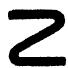
\includegraphics[keepaspectratio]{images/part001_9ca68205.jpg}}

注. 豪斯多夫空间可以是紧子空间的可数并而不是局部紧的。* 例如带弱拓扑的 Hilbert 空间便是如此，我们将在后续卷中证明这一点。

命题 15. 若 X 是局部紧 \(\sigma\) 紧空间，则存在 X 的相对紧开子集的一个序列 \((\mathbf{U}_n)\)，它覆盖 X，且 \(\overline{\mathbf{U}}_n \subset \mathbf{U}_{n+1}\) 对每个 \(n\) 成立。

设 X 是紧集序列 \((\mathbf{K}_{n})\) 的并。设 \(U_{1}\) 是 \(K_{1}\) 的一个相对紧开邻域（第 7 目，命题 10），并归纳地定义 \(U_{n}\)（对 n \textgreater{} 1）为 \(\overline{U}_{n-1} \in K_{n}\) 的一个相对紧开邻域（第 3 目，命题 5；第 7 目，命题 10）。序列 \((\mathbf{U}_{n})\) 显然具有所需的性质。

推论 1. 用命题 15 的记号，X 的每个紧子集 K 都包含于某个 \(U_{n}\) 中。

因为 K 可由有限多个 \(U_{k}\) 覆盖，依据公理 (C'\,')。

推论 2. 设 X 是局部紧空间，X' 是由 X 添加无穷远点 ω 而得到的紧空间（第 8 目）。则 X 是 σ 紧的，当且仅当点 ω 在 X' 中有一个可数的基本邻域系。

若 X 是 σ 紧的，我们可以如命题 15 那样构造 X 的子集序列 \(U_{n}\)，而诸邻域 \(X^{\prime}-\overline{U}_{n}\)（\(\omega\) 在 \(X^{\prime}\) 中的）依据推论 1 构成 \(\omega\) 的一个基本邻域系。反之由如下事实得出：\(\omega\) 的开邻域的余集是 X 的紧子集。

显然，局部紧 \(\sigma\) 紧空间的每个闭子空间都是局部紧且 \(\sigma\) 紧的。同样，局部紧 \(\sigma\) 紧空间的任意有限积是局部紧且 \(\sigma\) 紧的。

但要注意，紧空间的开子空间未必是 \(\sigma\) 紧的，正如 Alexandroff 定理（第 8 目，定理 4）所示。

